\begin{figure}[ht]
\begin{center}
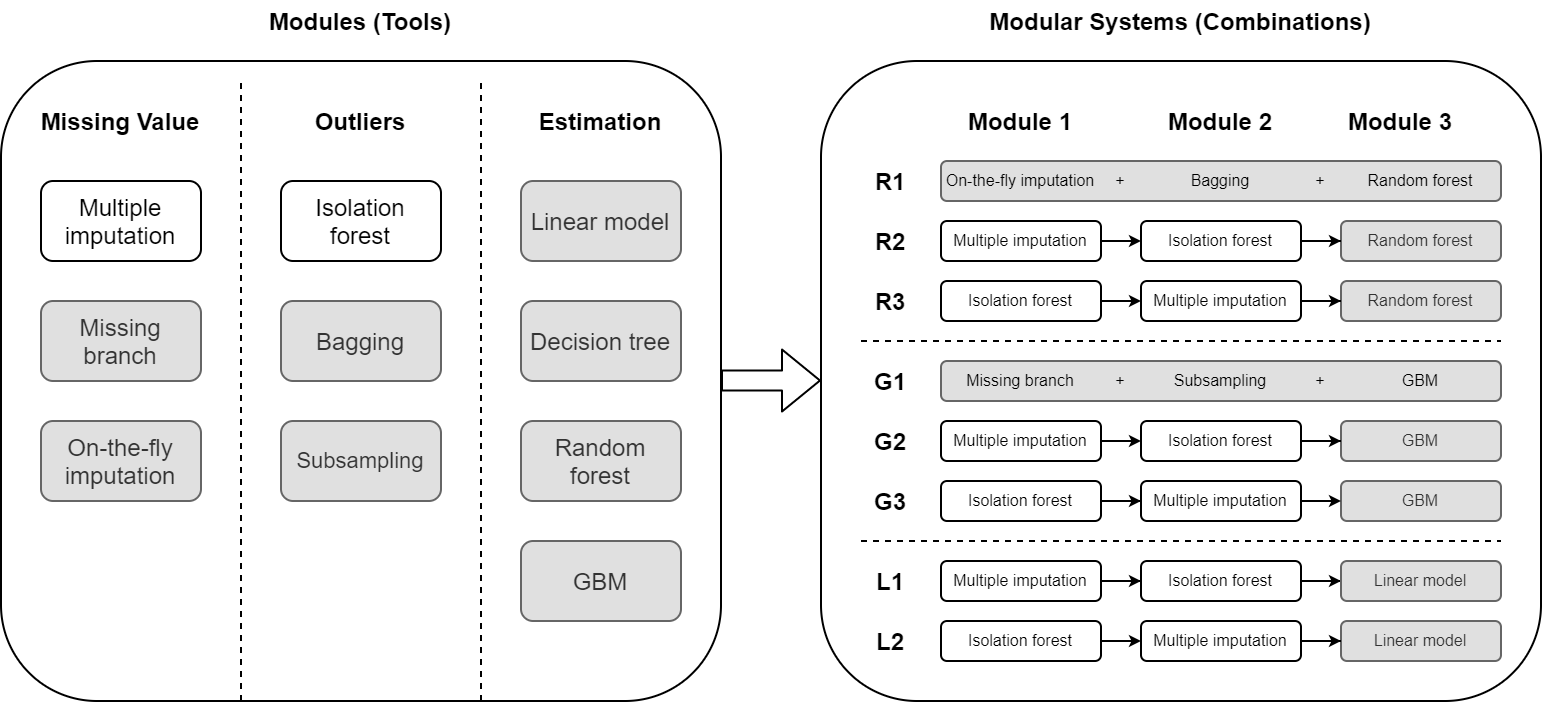
\includegraphics[scale=0.25]{./images/approach_tools}
\caption{{\bf The problem solving modules (tools) and the modular systems (combinations).} shows the combinations of different methods to be used in the process of developing modular systems of AVM. Each module only deals with one aspect of the prediction problem, missing values (M), outliers (O) or the estimation (E). The modules with gray background indicate that they could cooperate with estimation modules internally and simultaneously or they are estimation modules.\setlength{\baselineskip}{1.25em}}
\label{fig_approach_tools}
\end{center}
\end{figure}